\documentclass[exercice]{thedocument}%
\startdatakeys
\source{22GENMATPO1}
\cycle{4}
\competencesDuSocle{CA, CO}
\connaissancesRequises{A3b2}
\competencesTravaillees{A3a1,A3a3,A3b*}
\enddatakeys
\begin{document}%
On considère le programme de calcul suivant~:\par
\begin{center}
    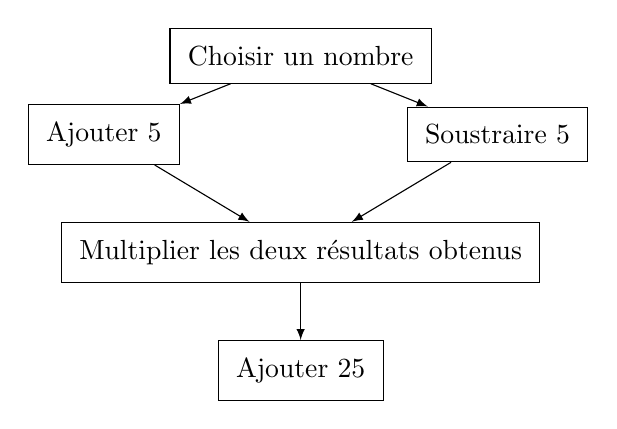
\begin{tikzpicture}
    \tikzset{%
        n/.style={draw, inner sep=1.5ex},
        e/.style={-latex}%
        }
    \node[n](a1)at(0,4){Choisir un nombre};
    \node[n](b1)at(-2.5,3){Ajouter 5};
    \node[n](b2)at(2.5,3){Soustraire 5};
    \node[n](c1)at(0,1.5){Multiplier les deux résultats obtenus};
    \node[n](d1)at(0,0){Ajouter 25};
    \path
    (a1)edge[e](b1)
    (a1)edge[e](b2)
    (b1)edge[e](c1)
    (b2)edge[e](c1)
    (c1)edge[e](d1);
    \end{tikzpicture}
\end{center}
\begin{enumerate}
    \item \begin{enumerate}
        \item Si on choisit le nombre 7, vérifier que l'on obtient 49
        à la fin du programme.
        \item Si on choisit le nombre -4, quel résultat obtient-on à
        la fin du programme~?
    \end{enumerate}
    \item On note $x$ le nombre choisi au départ.
    \begin{enumerate}
        \item Exprimer en fonction de $x$ le résultat obtenu.
        \item Développer et réduire $(x+5)(x-5)$.
        \item Sarah dit~:\guillemotleft\ Avec ce programme de calcul, quel
        que soit le nombre choisi au départ, le résultat obtenu est toujours
        le carré du nombre de départ.
        \guillemotright
    \end{enumerate}
\end{enumerate}
\showthesource
\end{document}
